% ---------------------------------------------------------------------
% captions.tex — main figure captions, main table, Extended Data captions
% ---------------------------------------------------------------------
\section*{Main figures and table}

\begin{figure}[htbp]
\centering
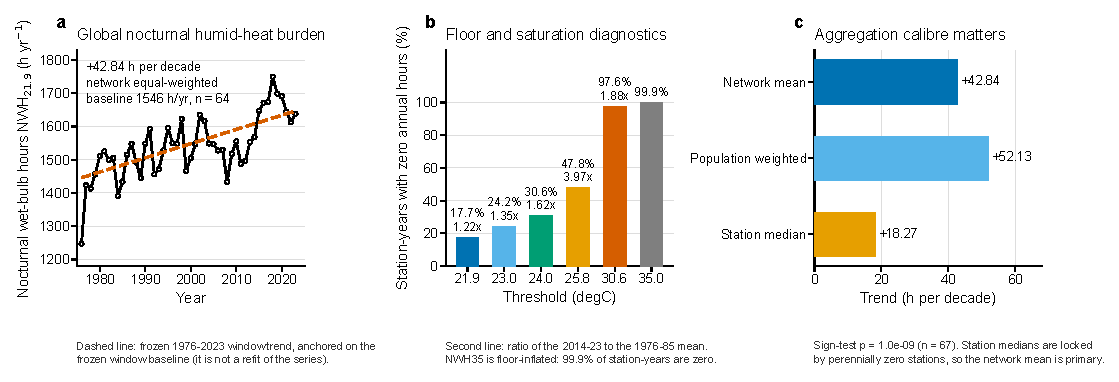
\includegraphics[width=\textwidth]{Fig1.pdf}
\caption{\textbf{Global night-time humid-heat burden and the choice of threshold.}
\textbf{a}, Annual network-mean night-time hours with wet-bulb temperature $\geq21.9$\,\dd{}
($\mathrm{NWH}_{21.9}$), 1976--2023, 64 stations with $\geq$90\% window coverage; dashed line is
the frozen window trend ($+42.84$\,h per decade) anchored on the 1976--85 baseline
(1,546\,h\,yr$^{-1}$). \textbf{b}, Zero-inflation diagnostic: share of station-years with zero
crossing hours (bars) and growth ratio of 2014--23 to 1976--85 means (labels) by threshold;
thresholds above 30\,\dd{} are floor-inflated. \textbf{c}, Aggregation calibre matters: network
mean ($+42.84$), population-weighted ($+52.13$) and station median ($+18.27$) trends on the
identical station set; the station median is locked by permanently zero stations, so the network
mean is primary.}
\label{fig:fig1}
\end{figure}

\begin{figure}[htbp]
\centering
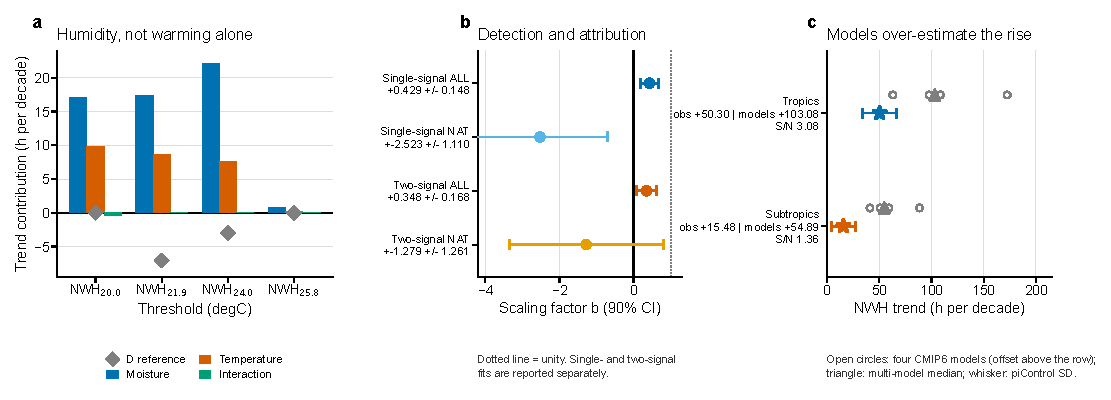
\includegraphics[width=\textwidth]{Fig2.pdf}
\caption{\textbf{Humidity necessity and anthropogenic detection.}
\textbf{a}, Variance-preserving counterfactual decomposition of the $\mathrm{NWH}_{21.9}$ trend by
threshold (station-median calibre, $n=72$): moisture (blue), temperature (orange), interaction
(green), double-detrended reference (diamond). \textbf{b}, Optimal-fingerprint scaling factors with
90\% confidence intervals: single-signal ALL ($+0.429\pm0.148$), single-signal NAT (rejected),
two-signal ALL ($+0.348\pm0.168$) and two-signal NAT. \textbf{c}, Observed versus CMIP6
$\mathrm{NWH}$ trends (h per decade): open circles, individual models; triangles, multi-model
median; whisker, piControl internal variability; observation-to-internal-variability ratios 3.08
(tropics) and 1.36 (subtropics).}
\label{fig:fig2}
\end{figure}

\begin{figure}[htbp]
\centering
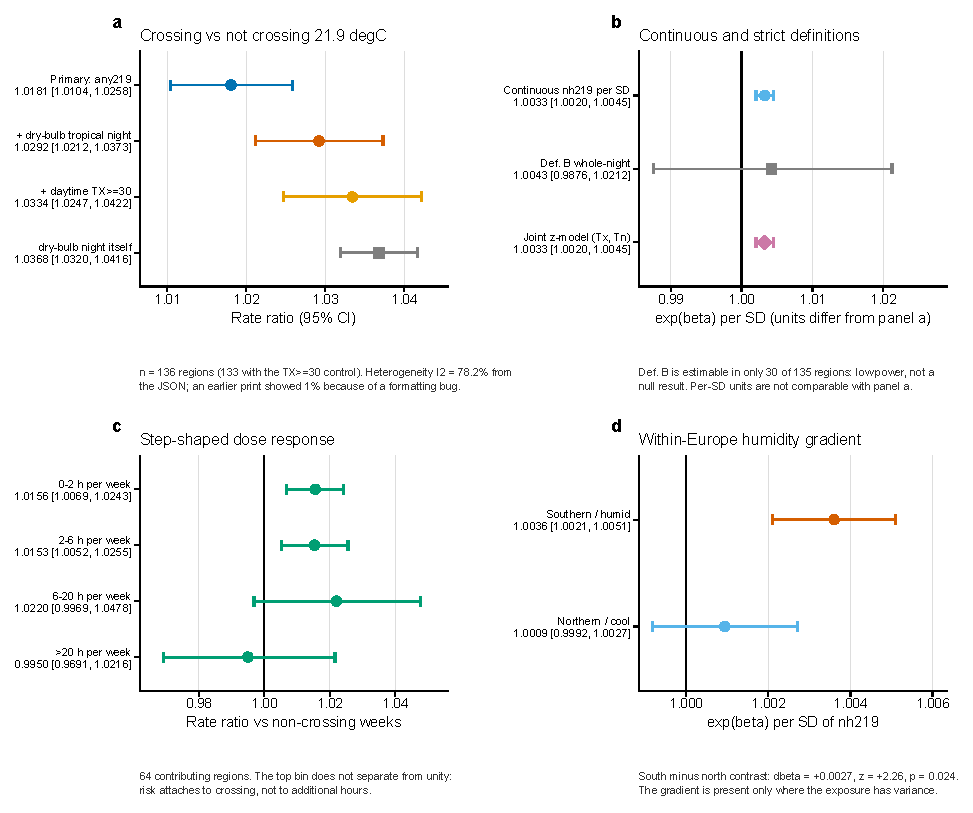
\includegraphics[width=\textwidth]{Fig3.pdf}
\caption{\textbf{Mortality attaches to the crossing event (Europe, weekly, 2001--2024).}
\textbf{a}, Rate ratios for weeks with any nocturnal hour $\geq21.9$\,\dd{}, alone and adjusted for
dry-bulb tropical nights or daytime TX $\geq30$\,\dd{} (136 regions; 133 with the TX control).
\textbf{b}, Continuous (per SD) and strict whole-night definitions; definition B is estimable in
only 30 regions (low power, not a null result). \textbf{c}, Dose--response by weekly crossing
hours: risk attaches to the first crossing and does not increase with additional hours.
\textbf{d}, Southern/humid versus northern/cool strata (per SD of continuous exposure); contrast
$z=+2.26$, $p=0.024$.}
\label{fig:fig3}
\end{figure}

\begin{figure}[htbp]
\centering
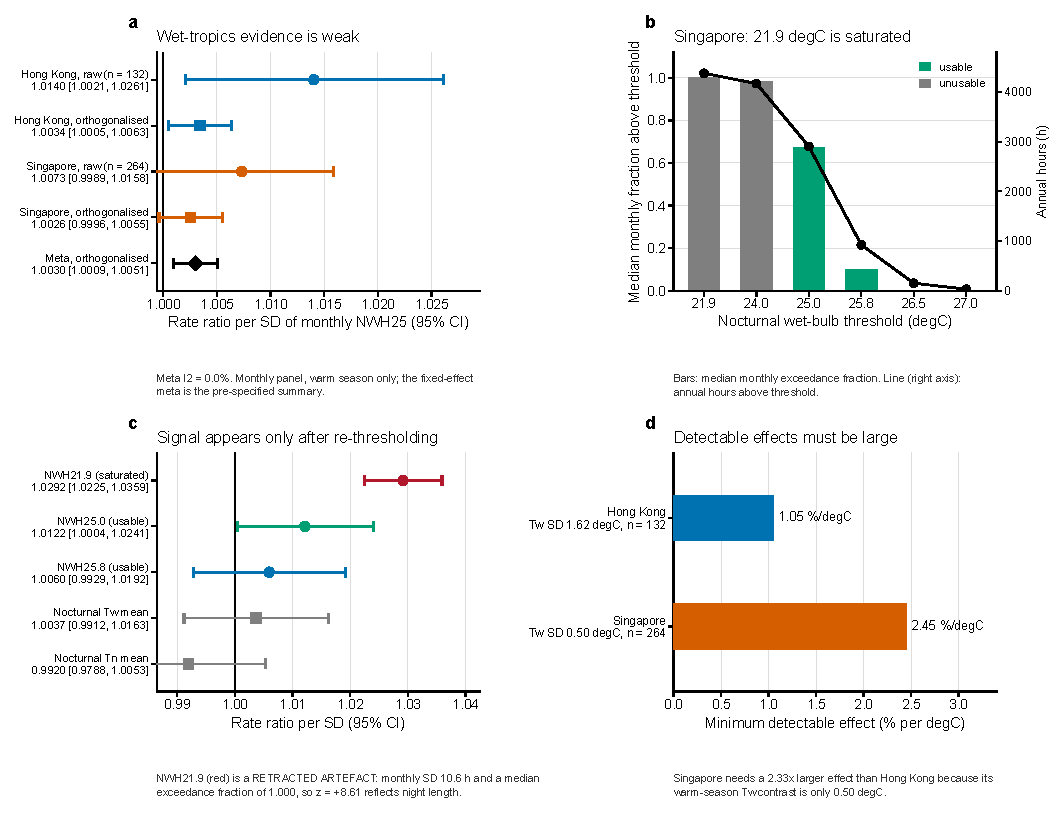
\includegraphics[width=\textwidth]{Fig4.pdf}
\caption{\textbf{Wet-tropics replication, threshold failure and statistical power.}
\textbf{a}, Monthly $\mathrm{NWH}_{25}$ mortality associations (rate ratio per SD, 95\% CI) for
Hong Kong ($n=132$ months) and Singapore ($n=264$), raw and dry-bulb-orthogonalised, with the
pre-specified random-effects meta-analysis ($I^2=0\%$). \textbf{b}, Singapore threshold
saturation: median monthly exceedance fraction (bars; usable in green) and annual crossing hours
(line, right axis); 21.9 and 24\,\dd{} are saturated. \textbf{c}, Re-thresholded models: the
$\mathrm{NWH}_{21.9}$ result (red) is a rejected saturation artefact (median exceedance fraction
1.000; $z=+8.61$ reflects night length); 25.0 and 25.8\,\dd{} are valid. \textbf{d}, Minimum
detectable effects: Singapore requires a $2.33\times$ larger true effect than Hong Kong because its
warm-season night-time $T_\mathrm{w}$ varies by only 0.50\,\dd{} (SD) versus 1.62\,\dd{}.}
\label{fig:fig4}
\end{figure}

\begin{figure}[htbp]
\centering
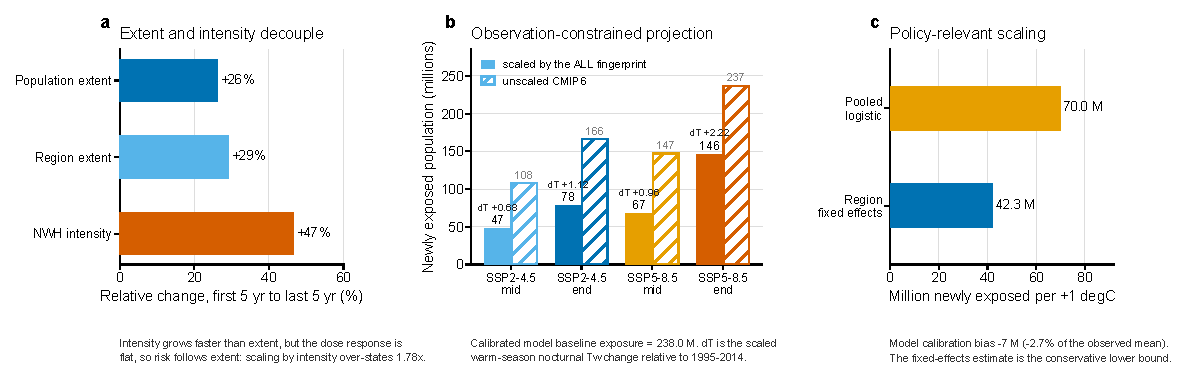
\includegraphics[width=\textwidth]{Fig5.pdf}
\caption{\textbf{Extent--intensity decoupling and observation-constrained projections.}
\textbf{a}, Relative change between the first and last five years of 2000--2024 in exposed
population ($+26\%$), exposed regions ($+29\%$) and mean crossing hours ($+47\%$); because the
dose--response is flat beyond the first crossing, scaling risk by intensity overstates
risk-relevant growth $1.78\times$. \textbf{b}, Newly exposed European population (millions) under
SSP2-4.5 and SSP5-8.5 at mid- and end-century, fingerprint-scaled (solid) versus unscaled CMIP6
(hatched); $\Delta T$ is the scaled warm-season night-time $T_\mathrm{w}$ change relative to
1995--2014. \textbf{c}, Policy-relevant scaling: millions newly exposed per $+1$\,\dd{} of
warm-season night-time $T_\mathrm{w}$ (pooled logistic $70.0$; region fixed effects $42.3$,
conservative); model calibration bias $-7$ million ($-2.7\%$ of the observed mean).}
\label{fig:fig5}
\end{figure}

\begin{table}[htbp]
\centering
\footnotesize
\caption{\textbf{Primary results and key sensitivities.} All values trace to frozen,
hash-verified artefacts (Extended Data Table~\ref{tab:edtable1} gives the complete register,
including retracted analyses that are never presented as results).}
\label{tab:main}
\begin{tabular}{p{5.2cm}p{4.0cm}p{6.2cm}l}
\toprule
Quantity & Sample & Effect (95\% CI unless stated) & Status \\
\midrule
$\mathrm{NWH}_{21.9}$ trend, 1976--2023 & 64 stations, network equal-weighted & $+42.84$\,h per decade; baseline 1,546\,h\,yr$^{-1}$ & Primary \\
Window sensitivity (8 windows) & balanced sets per window & $+27.69$ to $+58.62$\,h per decade, all positive & Sensitivity \\
Aggregation calibre & same 64 stations & $+42.84$ / $+52.13$ / $+18.27$ (mean / pop-weighted / median) & Sensitivity \\
Moisture necessity, $\mathrm{NWH}_{21.9}$ & 72 stations, S-calibre & warming-only $-6\%$; humidity requirement $+106\%$ & Primary \\
Optimal-fingerprint scaling & tropics + subtropics, 1976--2014 & $b_\mathrm{ALL}=+0.429\pm0.148$ (single); $+0.348\pm0.168$ (two-signal) & Primary \\
Mortality, crossing 21.9\,\dd{} (any219) & 136 regions, 77,551 region-weeks & RR $=1.0181$ $[1.0104,1.0258]$, $z=+4.62$, $I^2=78.2\%$; AF $=1.77\%$ $[1.02,2.52]$ & Primary \\
$+$ dry-bulb tropical-night control & 136 regions, joint model & any219 RR $=1.0292$ $[1.0212,1.0373]$, $z=+7.21$ & Identification test \\
Dose--response bins & 64 regions with graded exposure & 0--2\,h $1.0156$; $>$20\,h $0.9950$ ($z=-0.37$) & Step response \\
South--north Europe contrast & 101 / 35 regions & $1.0036$ vs $1.0009$ per SD; contrast $z=+2.26$, $p=0.024$ & Effect modification \\
Wet-tropics meta (orthogonalised) & HK 132 + SG 264 months & $1.0030$ $[1.0009,1.0051]$, $z=+2.83$, $I^2=0\%$ & Replication \\
Threshold saturation, Singapore & 300 months & exceedance fraction 1.000 (21.9\,\dd{}), 0.672 (25.0\,\dd{}) & Threshold failure \\
Minimum detectable effect, tropics & HK / SG & $1.05$ vs $2.45\%$ per \dd{} (ratio $2.33\times$) & Power diagnosis \\
Extent vs intensity, Europe & 135 regions, 2000--2024 & population $+26\%$, regions $+29\%$, NWH $+47\%$; overstatement $1.78\times$ & Primary \\
Newly exposed population & 135 regions, 499 million & SSP2-4.5 $+78$ M; SSP5-8.5 $+146$ M (end-century, scaled) & Primary \\
Exposure response per $+1$\,\dd & same sample & $70.0$ M pooled / $42.3$ M fixed effects & Primary \\
Implementation uncertainty & reference re-implementation & $u_c=35.7$--$39.0\%$; night definition dominates & Limitation \\
\bottomrule
\end{tabular}
\end{table}

\clearpage
\section*{Extended Data}

\begin{figure}[htbp]
\centering
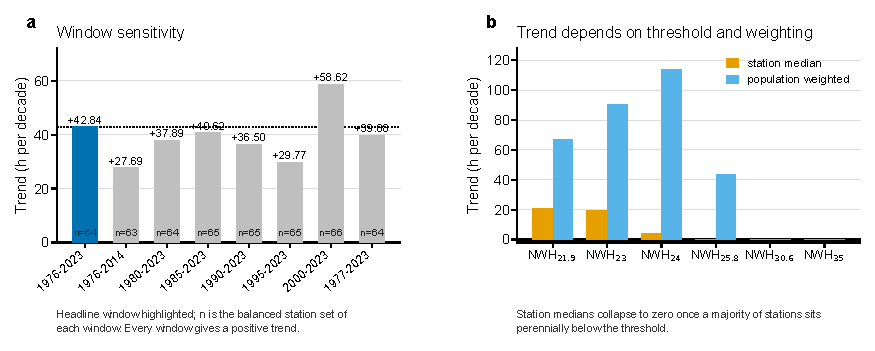
\includegraphics[width=\textwidth]{ExtendedDataFig1.pdf}
\caption{\textbf{Window robustness of the headline trend.} Theil--Sen trend of
$\mathrm{NWH}_{21.9}$ for eight start/end windows (1976--2023 headline); all windows are positive,
range $+27.69$ to $+58.62$\,h per decade.}
\label{fig:ed1}
\end{figure}

\begin{figure}[htbp]
\centering
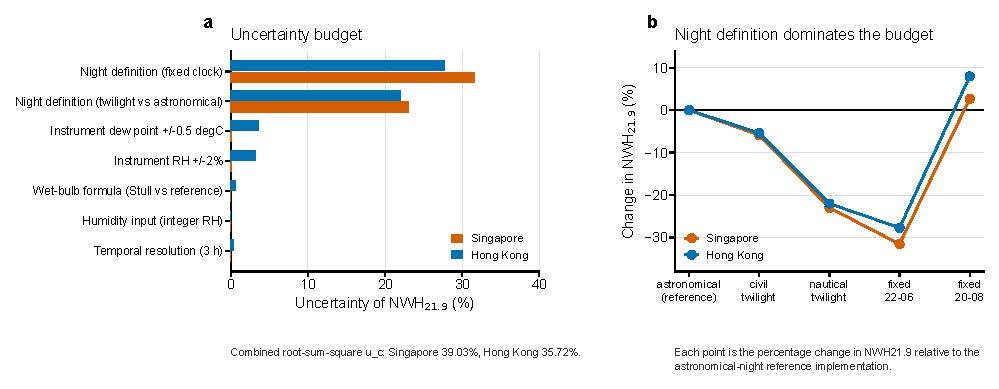
\includegraphics[width=\textwidth]{ExtendedDataFig2.pdf}
\caption{\textbf{Implementation uncertainty budget.} Component-wise and combined (root-sum-square)
relative uncertainty of the metric from a reference re-implementation at Hong Kong
($u_c=35.72\%$) and Singapore ($u_c=39.03\%$); the night definition dominates (22--32\%), wet-bulb
formula choice contributes $<0.6\%$.}
\label{fig:ed2}
\end{figure}

\begin{figure}[htbp]
\centering
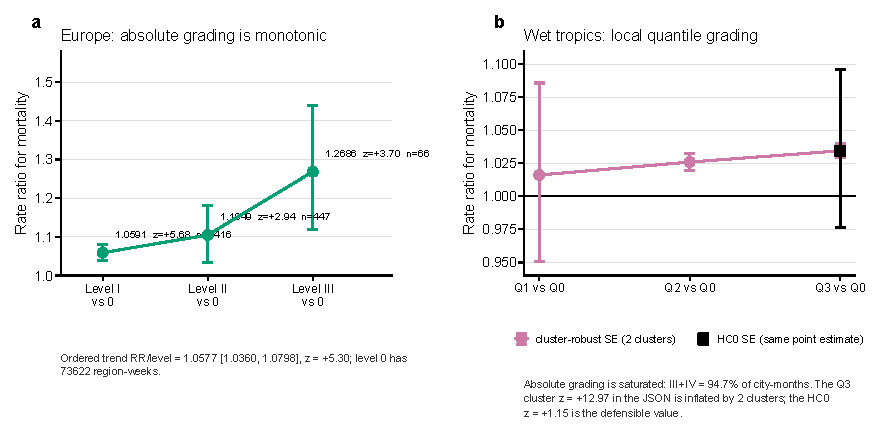
\includegraphics[width=\textwidth]{ExtendedDataFig3.pdf}
\caption{\textbf{Graded scale validation.} \textbf{a}, Mortality by graded level in Europe
(225 regions, 77,551 region-weeks): I $1.0591$ $[1.0384,1.0803]$, II $1.1049$ $[1.0338,1.1810]$,
III $1.2686$ $[1.1183,1.4391]$; monotone trend $1.0577$ per level, $z=+5.30$. \textbf{b}, Local
quantile grading in the wet tropics: with only two cities, cluster-robust SEs are unreliable and
HC0 intervals are reported alongside (Q3 HC0 CI $[0.9763,1.0962]$).}
\label{fig:ed3}
\end{figure}

\begin{figure}[htbp]
\centering
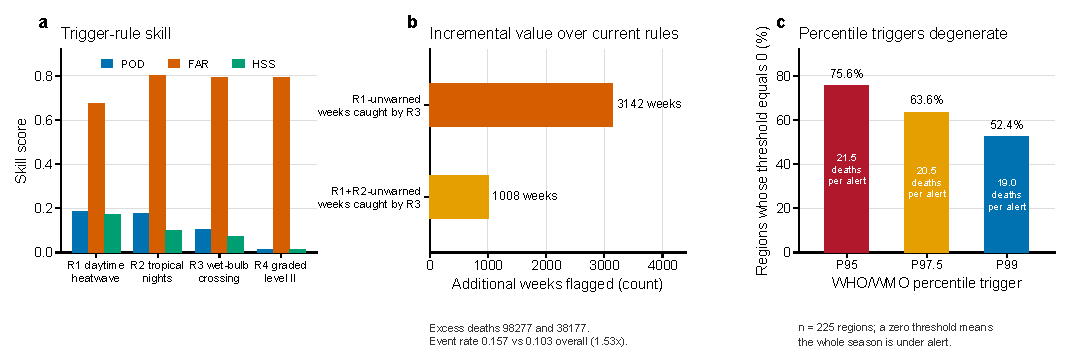
\includegraphics[width=\textwidth]{ExtendedDataFig4.pdf}
\caption{\textbf{Warning-skill evaluation and the percentile-trigger failure.} \textbf{a}, POD,
FAR and Heidke skill for four triggers; the nocturnal trigger alone (POD $0.102$) is below the
current daytime rule ($0.184$) and is positioned as an add-on. \textbf{b}, Incremental value:
3,142 weeks flagged only by the nocturnal trigger, event rate $1.53\times$ the panel average.
\textbf{c}, Zero-inflation failure of the WMO/WHO percentile default: the P95 (P97.5, P99)
warm-season $\mathrm{NWH}_{21.9}$ threshold equals zero in $75.6\%$ ($63.6\%$, $52.4\%$) of
European regions.}
\label{fig:ed4}
\end{figure}

\begin{figure}[htbp]
\centering
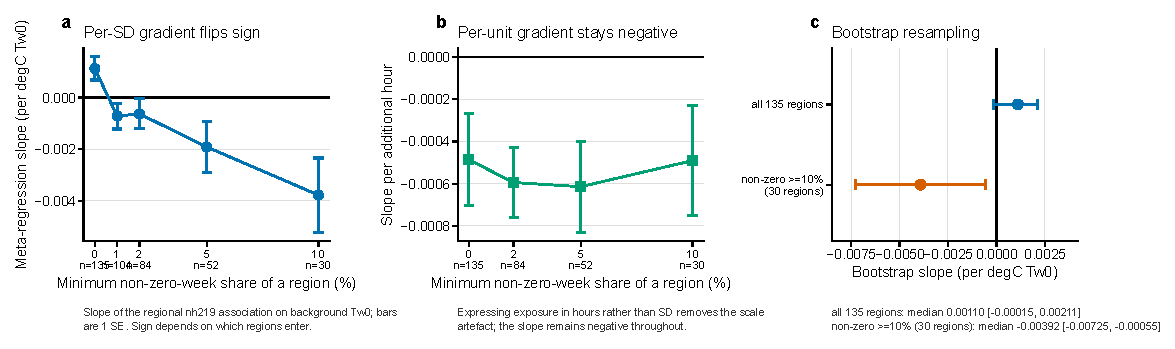
\includegraphics[width=\textwidth]{ExtendedDataFig5.pdf}
\caption{\textbf{Exposure--response gradient robustness.} Meta-regression of regional slopes on
background nocturnal $T_\mathrm{w}$: the unrestricted all-region slope is positive
($+0.00113$ per SD) but is driven by zero-variance regions; restricted to regions with non-zero
exposure in $\geq10\%$ of weeks the slope is negative ($-0.00377$); per-unit slopes are negative
throughout. Bootstrap intervals shown.}
\label{fig:ed5}
\end{figure}

\begin{figure}[htbp]
\centering
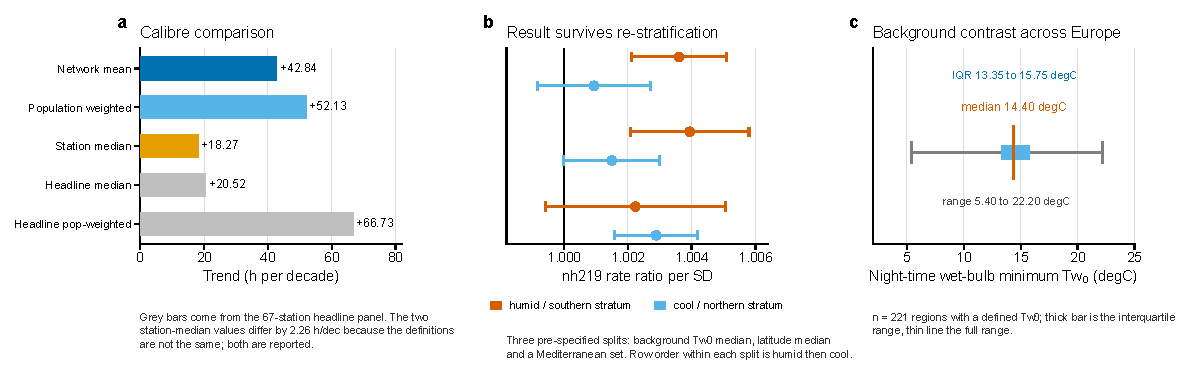
\includegraphics[width=\textwidth]{ExtendedDataFig6.pdf}
\caption{\textbf{Calibre and stratification robustness.} \textbf{a}, Two station-median
constructions of the headline trend (20.52 vs 18.27\,h per decade) are plotted side by side as
different estimators. \textbf{b}, The south--north contrast is stable across three stratification
schemes (background $T_\mathrm{w}$, latitude, Mediterranean): humid/southern strata 1.0036--1.0022
per SD versus cool/northern 1.0009--1.0015. \textbf{c}, Distribution of background warm-season
hottest-night wet-bulb minima across 221 regions (median 14.40\,\dd{}, IQR 13.35--15.75\,\dd{}).}
\label{fig:ed6}
\end{figure}

\clearpage
